\section{An overview of generative models}

\subsection{What is a Generative Model?}
In traditional, deterministic machine learning models (such as those used for classification or regression), the network learns a fixed function $y = f(x)$ that maps an input to a specific, constant output. We train these deterministic models by minimizing a point-wise loss function, such as the mean squared error, which explicitly compares the predicted output point with the ground truth target point. \\
Generative models, on the other hand, are inherently \textit{stochastic}: if we run the inference of the neural network $N$ times, we expect to generate $N$ different outputs. Because of this stochasticity, we can no longer evaluate the network by strictly comparing individual points; instead, we must compare probability distributions. We want the network to learn a generated probability density function $q(x)$ that matches the true data probability density function $p(x)$.

To achieve this, we need a loss function capable of measuring the difference between two distributions. A common choice is the \textbf{Kullback-Leibler (KL) divergence}. The KL divergence from $q$ to $p$ is defined as:
\begin{equation}\label{eq:KL_div}
    D_{KL}(p||q) = \int p(x) \log \frac{p(x)}{q(x)} dx = \mathbb{E}_{x \sim p} [\log p(x) - \log q(x)]
\end{equation}
It is important to note that the KL divergence is not a true mathematical distance (even though it effectively acts like a "distance between the two distributions") because it is not symmetric ($D_{KL}(p||q) \neq D_{KL}(q||p)$) and it does not satisfy the triangle inequality. Nevertheless, it is more than adequate for machine learning purposes. \\
Notice that with this choice we can actually treat our loss function as a functional (much like the action in Lagrangian mechanics) and apply variational principles to minimize it, ensuring that our model's distribution $q(x)$ converges to the true distribution $p(x)$. Of course $q(x)$ has the weights $w$ of the model as parameters. Since we must restrict $q(x)$ to be a valid probability density function (i.e., its integral must equal 1 and non-negative), a Lagrange multiplier is typically added to the loss formulation to bound the minimization:
\begin{equation}
    L[q]=D_{KL}(p||q) + \lambda \int q(x) dx
\end{equation}
We can now search for the minimum of $L[q]$:
\begin{equation*}
\begin{aligned}
    \delta L[q]=\int [p(x)\log p(x) &- p(x)\dfrac{1}{q(x)}] \ \delta q \ dx \ + \ \lambda \int \delta q \ dx \quad \Rightarrow \\
    \frac{\delta L[q]}{\delta q(x)} &= -\frac{p(x)}{q(x)} + \lambda = 0 \quad \Rightarrow
\end{aligned}
\end{equation*}
\begin{equation}
    q(x) = \frac{p(x)}{\lambda}
\end{equation}
To find the specific value of $\lambda$, we enforce the normalization constraint $\int q(x) dx = 1$:
\begin{equation*}
    \int \frac{p(x)}{\lambda} dx = 1 \quad \Rightarrow \quad \frac{1}{\lambda} \int p(x) dx = 1
\end{equation*}
Since $p(x)$ is the true data distribution, it is already a valid probability density function, meaning $\int p(x) dx = 1$. Therefore:
\begin{equation}
    \lambda = 1
\end{equation}
Substituting $\lambda = 1$ back into our stationary solution, we arrive at the \textit{theoretical global minimum}:
\begin{equation}
    q(x) = p(x)
\end{equation}
This analytical result demonstrates that minimizing the KL divergence under the normalization constraint guarantees that our generated distribution $q(x)$ converges exactly to the true data distribution $p(x)$.

\subsection{Autoencoders and Variational Autoencoders (VAEs)}
Before discussing pure generative models, let us briefly revisit the concept of dimensionality reduction. A classic technique is the Principal Component Analysis (PCA) we mentioned in the first section of the module, which diagonalizes the covariance matrix to find the directions of maximum variance. However, PCA is strictly limited to linear transformations (essentially rotating the axes). If your data lies on a complex, non-linear manifold (e.g., a circle), PCA will fail to capture the true underlying structure because it cannot perform the necessary non-linear transformations, like converting to polar coordinates.

Autoencoders solve this by using neural networks to perform non-linear dimensionality reduction. An autoencoder (represented below with a vector input) consists of an \textit{encoder} network that maps the high-dimensional input $x$ into a much smaller, low-dimensional \textit{latent representation} $z$, and a \textit{decoder} network that reconstructs the original input from $z$ as output $\hat{x}$. The network is trained using an unsupervised approach by minimizing the reconstruction error between the input and the output, so the loss function will be something like $L \sim (x-\hat{x})^2$.

\begin{center}
    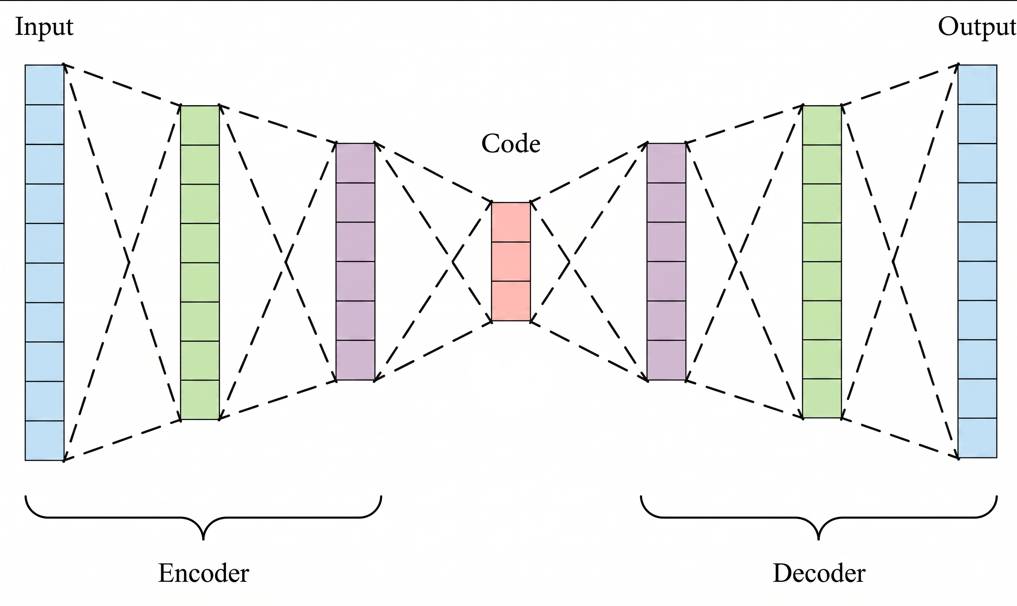
\includegraphics[width=0.6\textwidth]{figuresML/lesson_ml_5_pag_7.png}
\end{center}

The fundamental idea behind this architecture is to learn a meaningful representation of the data in the latent space $Z$ (e.g., defined by coordinates $z_1$ and $z_2$). For instance, if we train the autoencoder using images of dogs and cats as inputs, the network will learn to map these distinct classes to different, clustered regions within this latent space. The network effectively encodes the essential information required to reconstruct the output from the input, guided by the loss function.

Crucially, this process necessitates dimensionality reduction, often referred to as a bottleneck. Imagine if we were to design the architecture inversely: expanding the hidden layers so that the dimension of $Z$ is significantly larger than the input space $X$. This approach would fail because the neural network would simply learn the identity mapping, essentially approximating the function $f(x) = x$. The network could just pass the input image through without applying any meaningful filter, effectively turning off the redundant neurons. 

Therefore, the bottleneck forces the network to compress the data and extract the true underlying structure. As a natural consequence of this compression and subsequent reconstruction from the posterior, the quality of the reconstructed image $\hat{x}$ will inherently be slightly degraded compared to the original input.

However, a standard autoencoder is not a true generative model because the latent space $Z$ is not regularized. What does this mean? Knowing that the encoder maps the input $x$ into a single point in the latent space, if we sample a random point from the latter that lies between two encoded training examples (see figure), the decoder will likely produce nonsensical noise because it never learned what to do with that specific empty region of space. This makes extrapolation and interpolation in an unconstrained latent space highly unstable.

\begin{center}
    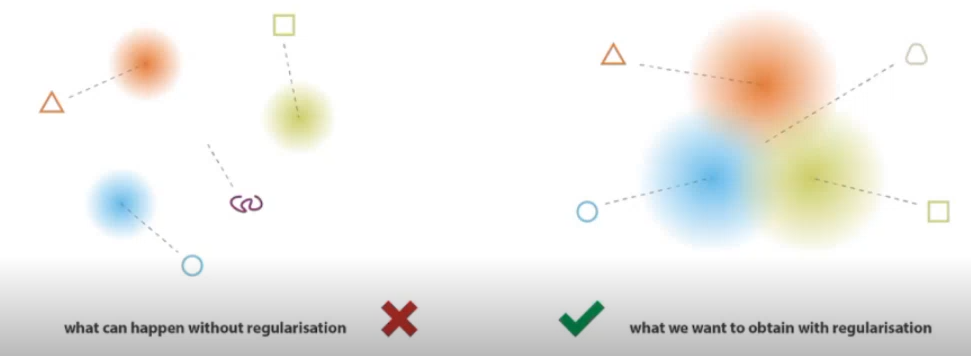
\includegraphics[width=0.7\textwidth]{figuresML/lesson_ml_5_pag_10.png}  
\end{center}

To make the autoencoder stochastic and fully generative, we use the \textbf{Variational Autoencoder (VAE)}. Instead of encoding an input $x$ into a single deterministic point $z$, the probabilistic encoder maps $x$ to the mean $\mu$ and standard deviation $\sigma$ of a Gaussian distribution, as shown in the following figure. We then sample the latent vector $z = \mu + \sigma \odot \epsilon$ (where $\epsilon \sim \mathcal{N}(0, I)$) and pass it to the decoder. By forcing the latent representations to follow a known distribution (like a Gaussian), we ensure the latent space is smooth and meaningful. This allows us to sample arbitrary points in the latent space and generate coherent, novel outputs, or gracefully interpolate between two different concepts. \\
To sum up, the key idea of VAEs is to introduce stochasticity during inference by regularizing the latent space ($\equiv$ "make it smooth"). We will take a look at the structure of a real-life VAE in the following hands-on section.

\begin{center}
    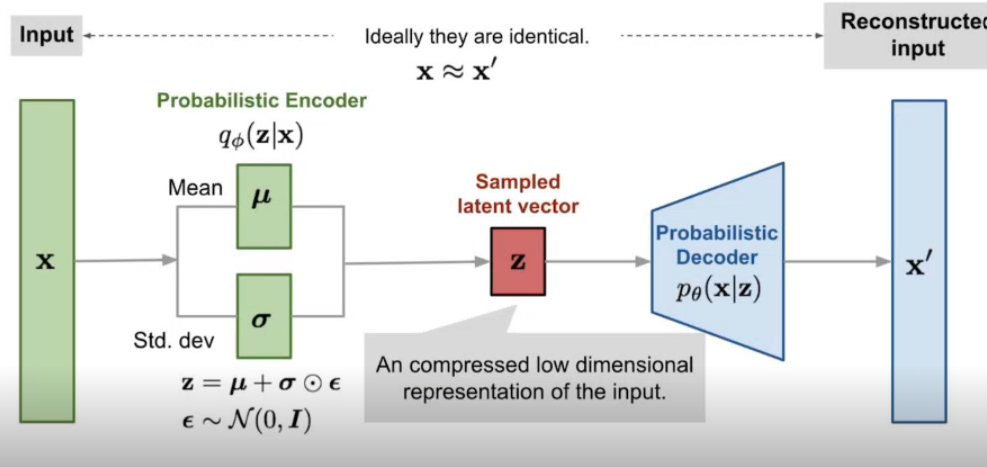
\includegraphics[width=0.8\textwidth]{figuresML/lesson_ml_5_pag_11.png}
\end{center}

Meaningful, smooth latent space representations are great for tasks like anomaly detection or data compression, and VAEs can interpolate between data points in a meaningful way in the latent space (e.g. you train your algorithm with images of cats and Van Gogh paintings, and you are able to generate an image of a cat painted in the style of Van Gogh). However, despite their elegance and flexibility, VAEs suffer from several known issues which are starting to make them obsolete:
\begin{itemize}
    \item[-] \textit{Mode collapse}: The model can generate a limited variety of outputs; 
    \item[-] \textit{Blurriness in outputs}: Due to dimensionality reduction, VAEs often produce blurrier results, especially in image generation tasks;
    \item[-] \textit{Complex training}: It is not easy to balance loss terms and regularize the phase space;
    \item[-] \textit{Limited expressiveness}: The assumption of a Gaussian prior limits the expressiveness of the model, impacting the variety of generated data.
\end{itemize}

\subsection{Generative Adversarial Networks (GANs)}\label{sec:intro_GAN}

\textbf{Generative Adversarial Networks (GANs)} represent a somewhat more "brute-force" approach to generation compared to the models discussed previously. The fundamental shift in this architecture is the origin of stochasticity: instead of injecting randomness into an intermediate latent space, it enters directly at the input stage, by feeding the network a random noise vector, which serves as the raw material for the generation process.

A GAN consists of two independent neural networks that work in tandem, effectively "competing" against each other:
\begin{itemize}
    \item[-] \textbf{Generator ($G$)}: This network takes the random noise vector $r$ and creates a synthetic data point, such as an image, effectively learning a function $G(r) = x_{\text{fake}}$. 
    %To force the generator to produce meaningful outputs rather than simply mapping noise to noise, it is pitted against an adversar.
    \item[-] \textbf{Discriminator ($D$)}: This network receives a mixture of real samples from the original training dataset and fake samples produced by the generator. Its objective is to correctly discriminate between them, assigning a label of real or fake.
\end{itemize}

\begin{center}
    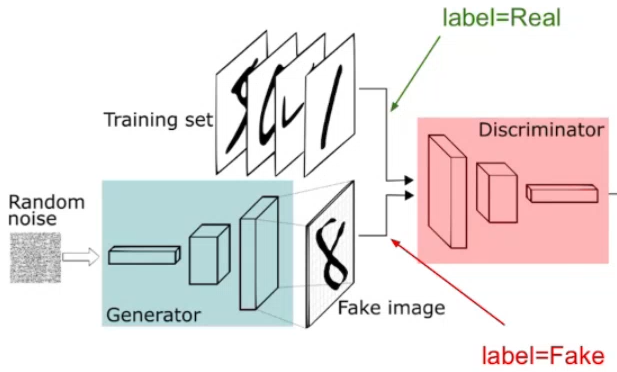
\includegraphics[width=0.6\textwidth]{figuresML/lesson_ml_5_pag_13.png}
\end{center}

At first glance, the discriminator's task appears to be a standard supervised learning problem because it relies on truth labels. However, the approach is fundamentally unsupervised because these labels are automatically defined by the system, so even if you inherently know which images were generated and which are from the true dataset, no manual annotation is needed.

The core dynamic of a GAN is defined as a \textbf{min-max problem}. The discriminator's goal is to distinguish the original training samples from the generated ones, maximizing its ability to catch fakes, while the generator attempts to fool the discriminator by creating increasingly realistic samples. Ultimately, this means minimizing a loss function with respect to the generator while maximizing a loss function with respect to the discriminator, driving both networks to continuously improve.

To understand how this tandem training works in practice, let's take a look at the mathematical formulation of the loss function. \\
The discriminator $D$ acts as a binary classifier whose output represents a probability that the given input is real, yielding a value between 0 and 1. Its goal is to maximize its accuracy, which translates to maximizing the following objective function:
\begin{equation}
    \max_D \mathcal{L}_D = \mathbb{E}_{x}[\log D(x)] + \mathbb{E}_{z}[\log(1 - D(G(z)))]
\end{equation}
We can break down the discriminator's logic into two distinct parts:
\begin{itemize}
    \item[-] For a real input $x$ from the training set, we want the discriminator to confidently predict 1. Therefore, we maximize the expected value of the logarithm of the discriminator's output, $\mathbb{E}_{x}[\log D(x)]$. 
    \item[-] For a fake image $G(z)$ generated from random noise $z$, we want the discriminator to confidently predict 0. This means minimizing the output $D(G(z))$, which is mathematically equivalent to maximizing the expected value of the complement, $\mathbb{E}_{z}[\log(1 - D(G(z)))]$. This conceptually aligns with penalizing the discriminator when it incorrectly labels a fake image as real.
\end{itemize}
Conversely, the generator $G$ is solely focused on fooling the discriminator. It wants the discriminator to output a value as close to 1 as possible for the fake images. Therefore, the generator's objective is to minimize the second term of the discriminator's loss:
\begin{equation}
    \min_G \mathcal{L}_G = \mathbb{E}_{z}[\log(1 - D(G(z)))]    
\end{equation}
When the generator is successfully minimizing this function, it implies that the discriminator is doing a poor job, meaning the generated images $G(z)$ look incredibly similar to the true input $x$. This is what we mean by a min-max problem: since the two networks are optimizing the same function in opposite directions, as training progresses the generator is forced to produce increasingly realistic structures to keep fooling an improving discriminator.

While GANs produce much sharper and more realistic images than VAEs since they are not subject to dimensionality reduction, their training dynamics are notoriously unstable. It is difficult to reach a good equilibrium between generator and discriminator, and GANs usually suffer from \textbf{mode collapse} (the generator might start producing the exact same realistic output repeatedly regardless of the input noise) and more importantly \textbf{vanishing gradient problems}. Intuitively, if the discriminator becomes too perfect too quickly, the generator receives no useful gradient information to improve its outputs.

To address the critical issue of vanishing gradients and training instability, instead of relying on a binary classification approach that minimizes a probabilistic divergence, an advanced formulation introduces concepts from the so-called \textit{Optimal Transport Theory}. In general, we seek the transformation $\mathcal{T}_{X \to Y}$ that requires the least number of steps ($\equiv$ the least amount of energy) to map a space $X$ to a space $Y$. In our case, this effort to minimize the transformation cost is formalized by the \textbf{Wasserstein Distance} (commonly known as the \textbf{Earth Mover's distance}), which provides a robust measure of the distance between the distribution of real data and the generated one. In this architecture, known as the \textbf{Wasserstein GAN (WGAN)}, the traditional discriminator is replaced by a \textbf{critic} network, denoted as $f_w(x)$ \footnote{A crucial mathematical requirement for this objective function to be valid is that the critic $f_w$ must be trained to learn a \textit{Lipschitz continuous} function. Although enforcing this Lipschitz constraint in practice is not trivial, the theoretical payoff is significant.}. Rather than outputting a probability bounded between 0 and 1, the critic outputs a raw scalar value that directly evaluates the similarity (or difference) between the distributions. The loss function is then entirely reconfigured to approximate this Wasserstein distance ($W$) between the real data distribution $p_r$ and the generated fake data distribution $p_g$:
\begin{equation}
    \mathcal{L}(p_r, p_g) = W(p_r, p_g) = \max_{w \in W} \left( \mathbb{E}_{x \sim p_r}[f_w(x)] - \mathbb{E}_{z \sim p_r(z)}[f_w(g_\theta(z))] \right)
\end{equation}
The Wasserstein distance provides a much smoother, linear gradient compared to regular GANs. This ensures that even when the fake and real distributions are entirely disjoint, the generator still receives a steady, meaningful gradient signal, effectively solving the vanishing gradient problem. Take a look at \url{https://arxiv.org/abs/1701.07875} and at the Advanced Machine Learning chapter for more details.

\subsection{Normalizing flows}
Another approach to work with probability density functions is the so-called \textbf{normalizing flows} technique. The idea is to apply a chain of simple, invertible transformations to map a simple base distribution (like a multi-dimensional Gaussian) into the complex target distribution of our data. The transformations must be bijective (invertible), so we can easily travel back and forth between the simple space $Z$ (controlled and defined by the user) and the complex data space $X$, allowing us to explicitly calculate the exact likelihood of the data. In other words, we are not actually learning the probability density function, but the function $f$ that will let us compute it point by point starting from a simpler one. Here is a simple representation:
\begin{center}
    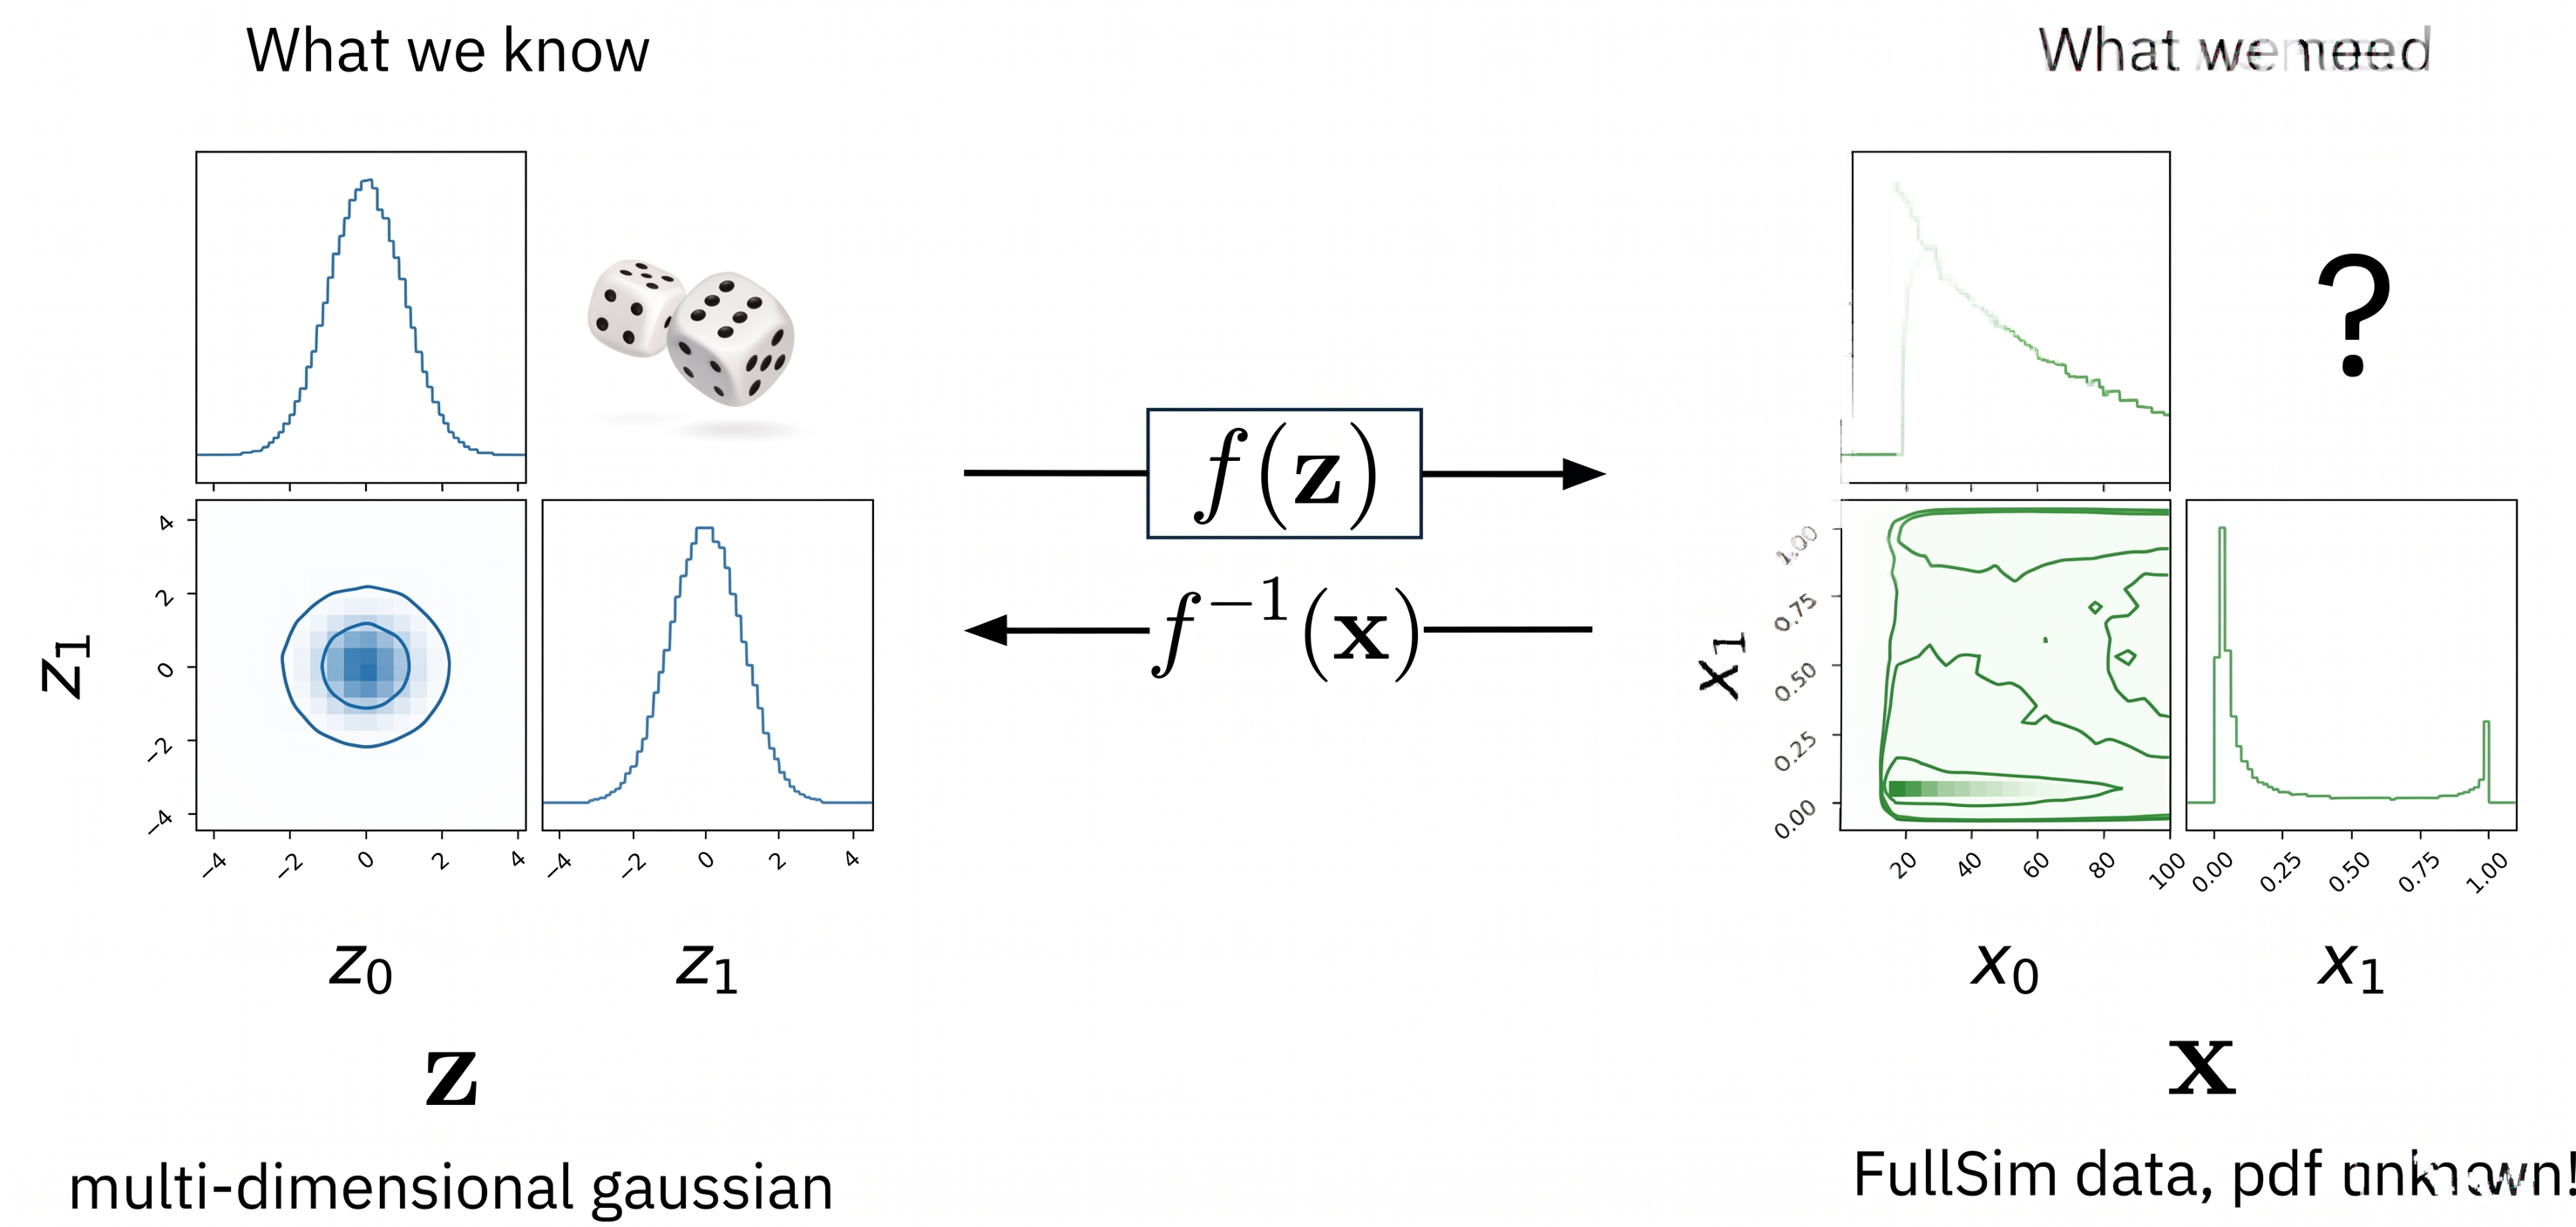
\includegraphics[width=0.8\textwidth]{figuresML/lesson_ml_5_pag_19.png}
\end{center}
There is an evident problem with this method: as you may imagine, inverting an arbitrary neural network is generally impossible. To maintain invertibility, normalizing flows rely on highly specific network architectures:
\begin{itemize}
    \item[-] \textbf{Autoregressive flows}: The network transforms variables sequentially. The first variable depends on nothing, the second depends only on the first, the third depends on the first and second, and so on (as shown below). This specific triangular structure makes calculating the Jacobian determinant and inverting the function computationally feasible.
    \begin{center}
        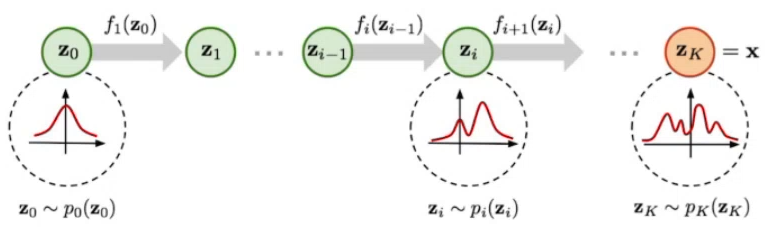
\includegraphics[width=0.8\textwidth]{figuresML/lesson_ml_5_pag_20.png}
    \end{center}
    \item[-] \textbf{Coupling layers}: The input vector is partitioned into two disjoint subsets, $x_A$ and $x_B$. The layer applies an identity mapping to one subset, while transforming the second subset using a function parameterized by a neural network conditioned on the first. Mathematically, the forward mapping to output $y = (y_A, y_B)$ is typically formulated as:
    \begin{equation*}
        \begin{cases}
            y_B = x_B \\
            y_A = x_A \cdot \exp(S(x_B))
        \end{cases}
    \end{equation*}
    where $S$ is an arbitrary neural network. The brilliance of this trick is its trivial invertibility: since $x_B$ is perfectly preserved as $y_B$, we can compute $S(y_B)$ and seamlessly apply the inverse operation (e.g., $x_A = y_A \cdot \exp(-S(y_B))$) to recover $x_A$ without ever needing to invert the neural network $S$ itself. To ensure the entire input space is fully transformed, consecutive coupling layers simply alternate which partition is passed through the identity mapping.
\end{itemize}

The modern evolution of this concept is known as \textbf{continuous flow}. Instead of relying on a sequence of discrete transformation layers to map a simple latent space to complex data, the process is modeled as a single, continuous transformation over time. 
The fundamental idea, trained via a technique called \textbf{flow matching}, is to start at time $t=0$ with a simple, easily sampleable distribution (like a Gaussian) and continuously morph it until $t=1$, where it matches the true target probability density function (p.d.f.):
\begin{equation*}
    \begin{cases}
        f(0; z) = z = \text{Gaussian} \\
        f(1; z) = \text{target p.d.f.}
    \end{cases}
\end{equation*}
To traverse this path, the variation of the distribution over an infinitesimal time step $dt$ is governed by a vector field, which effectively acts as the velocity required to move from the latent space $Z$ to the data space $X$. The DNN is explicitly tasked with learning this velocity field. Therefore, the continuous transformation can be described by the following differential equation:
\begin{equation*}
    f(t + dt) = f(t) + \text{DNN}(f(t)) \cdot dt
\end{equation*}
By integrating this learned velocity field over time, the model smoothly and efficiently transforms the random noise into the complex target distribution.

Another highly popular modern approach is \textbf{diffusion models}, which gradually add Gaussian noise to an image until it is completely destroyed, and then train a network to reverse the process, denoising the image step by step to generate new samples.

This was just a brief introduction to such methods, and we will dive a lot deeper into all the different flows and architectures summed up in the figure below during the Advanced Machine Learning chapter.

\begin{center}
    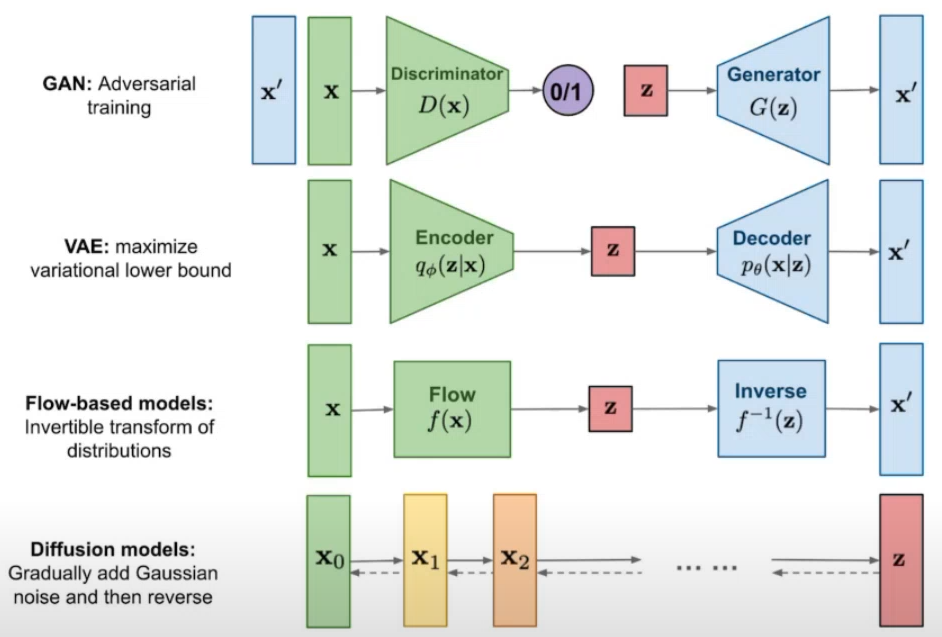
\includegraphics[width=0.65\textwidth]{figuresML/lesson_ml_5_pag_22.png}
\end{center}

\section{Hands-on example for Variational Autoencoders}

It is time to show how a Variational Autoencoder works in practice. Try to run the following Notebook by yourself, adjust the parameters and adapt it to different shapes.

You can find it here: \url{https://colab.research.google.com/drive/1TmONF8GWFJWSIn-3rDZEI_zV_NGccbbI?usp=sharing}.

%\includepdf[pages=-, pagecommand={\thispagestyle{plain}}]{lezioni/d_ML5_SOL.pdf} 

%ML_4 nel mio colab